\chapter{系统软件}


\section{uCore-thumips操作系统}
\label{section:ucore-thumips}
\subsection{系统概述}

uCore-thumips\footnote{\url{https://github.com/z4yx/ucore-thumips}} 是针对简化后的 MIPS 32 实现:MIPS32S 平台的 uCore 移植版本。该项目针对 MIPS32S 平台实现了对应的Bootloader、初始化流程、异常处理、内存管理和上下文切换流程。相比标准的 MIPS 32,MIPS32S 缺少部分指令且不支持延迟槽。针对这些不同,uCore-thumips 对 uCore 操作系统的编译选项进行了相应的修改,并提供了额外的库函数实现缺失的指令(如 \texttt{divu})的功能。

\subsection{编译方法}
在非 mipsel 平台编译、调试 uCore-thumips 需要使用面向 mipsel 架构的交叉编译、调试工具链,所需工具主要包括 binutils、gcc和gdb。

Debian 系统下,\texttt{gcc-mipsel-linux-gnu}和\texttt{binutils-mipsel-linux-gnu}软件包分别提供了预编译的目标平台为 mipsel 的 binutils 和 gcc。其它操作系统的工具链可参考 LinuxMIPS 项目文档\footnote{\url{https://www.linux-mips.org/wiki/Toolchains}}自行编译。此外 Sourcery CodeBench Lite\footnote{\url{https://sourcery.mentor.com/GNUToolchain/release2189}} 提供了预编译的 mipsel 工具链。 

交叉编译时,指定 \texttt{CROSS\_COMPILE} 环境变量或修改 Makefile 中 \texttt{CROSS\_COMPILE} 变量为所使用的交叉编译器,即可使用 make 进行编译。编译后得到镜像 \texttt{ucore-kernel-initrd} 和 \texttt{boot/loader.bin} 分别为系统内核 ELF 和Bootloader。

进行移植时,需针对片上系统对 Makefile 中相应配置进行修改,包括延迟槽、浮点模块等编译选项、为用户 App 预留存储大小等。

\subsection{系统分析}

\subsubsection{启动流程}
uCore-thumips 的引导、启动流程主要分为Bootloader加载系统、初始化C环境、初始化系统三个步骤。

uCore-thumips 提供了简易的Bootloader \texttt{boot/bootasm.S},该程序从 Flash(默认为地址0xBE000000)读取合法的ELF文件头,将其复制到内存的相应位置并跳转。

Bootloader加载系统后将跳转至 \texttt{kern/init/entry.S} 中的 \texttt{kernel\_entry} 过程。在此过程中,系统将重置 CP0 中异常相关寄存器、设置 TLB 相关异常向量;同时,正确设置 \texttt{sp, gp},清空\texttt{bss}以满足C程序运行要求,之后跳转至 \texttt{kern/init/init.c} 中的 \texttt{kern\_init} 函数。\texttt{kern\_init} 函数将完成中断控制、控制台、异常、内存管理、进程管理等系统功能的初始化。

进行移植时,需将Bootloader替换为针对NonTrivialMIPS片上系统自行实现的TrivialBootloader或U-Boot,针对平台对中断控制、控制台等功能的初始化过程进行相应修改。

\subsubsection{内存管理}

MIPS32 使用软件进行 TLB 缺失处理,当发生 TLB 缺失时会触发 TLB Refill 异常。uCore-thumips 已经实现了 TLB Refill 异常的处理。发生 TLB 缺失时,系统会首先检查页表判断是否为缺页,若为缺页调用 \texttt{do\_pgfault} 进行处理,否则检查权限后填充 TLB 表项。

\subsubsection{异常处理}
异常处理程序通过访问 CP0 中的 Cause 寄存器获取异常信息,同时需要正确设置 Status 寄存器中的某些位。用户态和特权态切换时,uCore 内核使用 \texttt{trapframe} 结构存储程序运行状况。uCore-thumips 已实现和 CP0 中寄存器的交互及\texttt{trapframe}的保存。

\subsection{移植内容}

\subsubsection{编译选项}
针对 NonTrivialMIPS 平台,我们对原版 ucore-thumips 的 Makefile 进行了如下修改。由于 NonTrivialMIPS 平台实现了 CP1 浮点运算协处理器,我们关闭了编译选项中软浮点数的开关;由于 CPU 支持延迟槽,我们允许编译器在延迟槽中生成代码。

\subsubsection{外设配置}
为使 uCore 正确操作外设,我们对外设相关常量进行配置。相关常量集中在内核源码中的头文件 \texttt{kern/include/thumips.h},修改的常量包括串口、等设备对应的内存地址,以及串口、时钟等设备的 IRQ 号。

% \subsubsection{键盘驱动}
% 我们引入了张宇翔助教移植的 USB 键盘驱动。该驱动的主体部分是@a1exwang\footnote{\url{https://github.com/a1exwang}} 同学编写的通过 SL811 USB 控制器与键盘进行交互的程序。宇翔助教的移植工作主要包括在 uCore 系统启动时对 USB 控制器进行初始化,以及在内核中创建线程,将读到的输入放入标准输入设备中。引入该驱动时只需将设备地址及CPU时钟频率等常量修改为 NonTrivialMIPS 平台对应的值。

\subsubsection{内存管理}
我们修改了 uCore 的 TLB 替换策略,轮流选择TLB项进行替换,使用 \texttt{tlbwi}指令。对 TLB 进行 reset 时,也将 TLB 的项数改为实际的项数。

另外,在移植过程中,我们发现了uCore存在的一个问题。在进程内存管理组件 \texttt{pmm.c} 的内存拷贝函数 \texttt{copy\_range} 中,如果内存不足导致分配的 \texttt{npage} 为空,原本的实现会直接导致内核崩溃。根据系统 API 语义,此时实际应该返回 \texttt{-E\_NO\_MEM}。按此修复后,系统内核不会在应用程序申请较多内存导致内存不足时崩溃,而是会正确地杀死用户态程序。

\subsection{新增内容}

\subsubsection{ulib字符输入库函数}
ulib 中只实现了字符输出的库函数,没有实现输入的相关函数。为了使用户态程序可以方便地与用户交互,我们为 ulib 增加了 \texttt{fgetch}、\texttt{getchar}以及\texttt{readint} 三个库函数。\texttt{fgetch}从指定文件读取一个字符,\texttt{getchar}从标准输入读入一个字符,\texttt{readint}从标准输入读入一个十进制整数。

\subsubsection{外设通信与系统调用}

外设所映射到的内存地址在内核态无法访问,为此需在内核中增加访问外设的系统调用。我们加入了\texttt{sys\_pread}和\texttt{sys\_pwrite}两个通用的外设访问系统调用。其中\texttt{sys\_pread}从外设读取数据,传入的参数以此为外设序号、读取数据的目的地址、读取数据的长度;\texttt{sys\_pwrite}将数据写入外设,传入的参数为外设序号、写入数据的来源地址、写入数据的长度。在 ulib 中,我们也加入了对这两个系统调用的封装,便于用户态程序使用。我们额外在 ulib 中加入了对硬件计时器访问的封装\texttt{int check\_timer(uint32\_t* time)}与\texttt{int set\_timer(uint32\_t time)}。

% 为了提高图形显示的速度,我们在MMU中降低了帧缓冲区的访问权限,从而使得用户态程序可以不经过系统调用,直接修改帧缓冲区。

\subsubsection{Mandelbrot 集绘制演示程序}

Mandelbrot 集指是的 $z_0 = 0,~z_{n+1} = z_n^2+c$ 收敛的复数$c$的集合。我们在 uCore 用户态实现了绘制 Mandelbrot 集的演示程序,用以验证 NonTrivialMIPS 平台的浮点计算及图像输出能力。可证明,若$c$属于Mandelbrot 集,则$|z_n|\leq 2$。在实际计算时,若经过\texttt{maxIteration}次迭代仍有$|z_n|\leq 2$,则近似认为$c$属于Mandelbrot 集。对于平面上的每个点$c$,将使得$|z_n|> 2$的最小的$n$映射到可显示的256种颜色之一,即可绘制Mandelbrot 集的图像。

利用ulib中新增的字符输入库函数,该演示程序可与用户交互,用户通过按键进行图像的平移与缩放。

\subsubsection{视频播放演示程序}

我们实现了一个简单的视频播放演示程序,可以从 Flash 中读取视频文件,输出到帧缓冲区中显示。我们首先对图像进行二值化,用1个bit表示一个像素,之后使用基于LZ77的压缩算法对二值化后的视频进行压缩。压缩算法的原理为,维护一个固定长度的窗口,从窗口中找到接下来输入中的最长匹配,用最长匹配在窗口中的位置、长度以及下一个字节表示这一最长匹配,最后将最长匹配加入窗口。伪代码如下:

\begin{minted}{python}
triplets = []
window = Queue(maxlen=WIN_SIZE)
i = 0
while i < len(data):
    for j in range(i+WIN_SIZE, i, -1):
        if data[i: j] in window:
            offset = window.index_of(data[i: j])
            length = j - i
            break
    triplets.append((offset, length, data[j]))
    window.push_back(data[i:j])
    i += length

\end{minted}

解压过程是压缩过程的逆过程,这里不再叙述。实际实现时,三元组中的每个元素都用8位固定长度整数存储,\texttt{WIN\_SIZE}取255。最终压缩后,视频体积为原二值化视频的4\%,长度为30s、帧率15fps、分辨率为800*600的黑白视频体积为1MB。

\subsubsection{幻灯片播放程序}

在视频播放的基础上,我们编写了幻灯片播放程序。与视频播放的不同之处在于,为实现前后翻页,幻灯片的每一页都分别进行压缩,并在文件头部依次以8位无符号数保存总页数及各页数据长度。另外,幻灯片的色彩为4位灰度,使用2个二进制位表示一个像素。


\section{Decaf教学编程语言}

\subsection{概述}
Decaf 是编译原理课程使用的实验性编程语言,编译原理课程提供了 Java 编写的 Decaf 编译器,能将 Decaf 源文件编译为 MIPS32 平台汇编。我们对操作系统、编译器进行了一些修改,使得 Decaf 程序可以在 uCore 的用户态正确运行。由于NonTrivialMIPS实现了完整的MIPS32 Rev I指令集,我们无需对编译器后端指令生成部分进行修改,主要工作集中于适配 Decaf 标准库。

最终,我们在NonTrivialMIPS平台上成功运行了\texttt{blackjack, math, nqueens, fibonacci} 四个 Decaf 应用程序。

\subsection{Decaf标准库移植}
Decaf 中涉及到与操作系统交互的部分为8个标准库函数,定义与功能详见表\ref{table:decaf_stl}。

\begin{table}[htbp]
    \centering
    \caption{Decaf标准库函数}
    \label{table:decaf_stl}
\begin{tabular}{|l|l|}
\hline
名称 & 功能 \\ \hline
Allocate & 分配内存,如果失败则自动退出程序 \\ \hline
ReadLine & 读取一行字符串(最大 63 个字符) \\ \hline
ReadInt & 读取一个整数 \\ \hline
StringEqual & 比较两个字符串 \\ \hline
PrintInt & 打印一个整数 \\ \hline
PrintString & 打印一个字符串 \\ \hline
PrintBool & 打印一个布尔值 \\ \hline
Halt & 结束程序 \\ \hline
\end{tabular}
\end{table}

为使得 Decaf 程序正确运行,需要为 uCore 系统构建 Decaf 标准库。我们选择将 libdecaf\footnote{\url{https://github.com/z4yx/libdecaf}} 移植到 uCore 平台。在 libdecaf 中,我们使用C语言,通过调用ulib中的相关函数,实现 Decaf 程序的输入、输出、退出功能,具体层次结构见图\ref{figure:libdecaf}。

\begin{figure}[htbp]
    \centering
    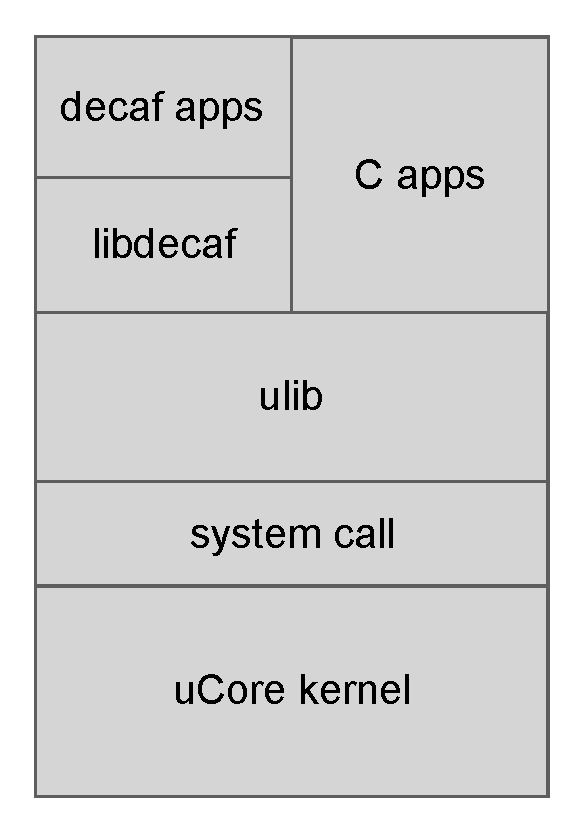
\includegraphics[width=0.3\linewidth]{decaf.pdf}
    \caption{Decaf标准库实现层次结构}
    \label{figure:libdecaf}
\end{figure}

Allocate在ulib中没有对应的实现。由于Decaf只分配内存而不释放,我们在libdecaf的中增加了一个静态数组作为Decaf程序的堆,调用Allocate时,首先将长度进行四字节对齐,然后返回数组相应元素的地址。

\subsection{与平台约定衔接}
Decaf 进行函数调用时,会将参数从右到左依次压入栈中,而在uCore系统中前四个参数分别保存在a0到a3寄存器中,其余参数压入栈中。因此,为了使得 Decaf 程序能够调用 C 编写的 libdecaf 中的函数,需对 Decaf 的标准库函数调用进行封装。我们使用汇编语言编写标准库函数调用的封装(\texttt{decafCall.S}),在调用时将参数从栈中取出,保存在对应的寄存器中,然后调用libdecaf的对应函数,以完成ABI的转换。以 \texttt{PrintString} 函数为例,核心代码如下所示。

\begin{minted}{asm}
    .type    __c_call, @function
__c_call:
    addiu   $sp, $sp, -20
    sw      $ra, 16($sp)
    la      $ra, __c_call_after_call
    jr      $t0

    __c_call_after_call:
    lw      $ra, 16($sp)
    addiu   $sp, $sp, 20
    jr      $ra


    .type   _PrintString, @function
_PrintString:
    lw      $a0, 4($sp)
    la      $t0, __decaf_printString
    j       __c_call
\end{minted}

uCore的用户态程序正常退出时应返回(在v0寄存器中保存)0,而Decaf程序的主函数没有返回值。为使其正确返回0,我们修改了 Decaf 编译器的后端,将Decaf程序主函数的名称修改为\texttt{\_\_decaf\_main}。同时,在 libdecaf 中加入main函数,调用\texttt{\_\_decaf\_main}并返回0。

我们将 Decaf 程序的编译加入了uCore系统的编译过程。在编译用户态程序时,首先检查\texttt{user}目录下是否存在Decaf源文件,若存在则调用编译原理课程提供的Decaf编译器将源文件编译为MIPS汇编,进而使用汇编器将其转换为目标文件,目标文件与 libdecaf 和 ulib 链接。uCore 中的用户态程序的入口为 ulib 中的 \texttt{umain} 函数,这一点通过在链接时指定链接脚本 \texttt{user/libs/user.ld} 完成。

\section{Linux操作系统}

Linux 是最为著名的开源操作系统,有丰富的软硬件支持。我们以 Linux 最新的稳定版本(v5.2.8)作为基线进行移植。

\subsection{CPU适配}

我们以 Linux 内核内置的 MIPS 4Kc CPU 为基础来实现移植,这是一款标准的 MIPS32 R1 CPU。首先我们需要添加 \texttt{TRIVIALMIPS} 这个架构,而后添加对应的架构目录(参见其他架构和 CPU 的目录结构即可)。

由于我们的 CPU 缺少一些功能(如 \texttt{Watch} 寄存器和 \texttt{PERF} 指令等),我们可以通过两种方式去除 Linux 的依赖。一方面,在 \texttt{arch/mips/include/asm/mach-trivialmips/} 目录下的 \texttt{cpu-features-overrides.h} 中可以通过定义类似 \texttt{cpu\_has\_watch} 的宏为 0,去除一些特定指令;另一方面,可以通过 \texttt{arch/mips/trivialmips/Platform} 文件来指定编译选项,如使用 \texttt{-mno-branch-likely} 去除 Branch Likely 等未实现的指令。

由于 NonTrivialMIPS 按照规范实现了 TLB 相关的 CP0 寄存器(包括 \texttt{Index, Wired, EntryHi, EntryLo, Random, PageMask} 等)与指令(包括 \texttt{TLBWI, TLBWR, TLBR} 等),因此无需修改 Linux 进程调度修改的代码。此外,Linux 也能够正常从 CP0 的 \texttt{Config1} 寄存器中得到 Cache 的相关属性(如大小、相连度)。对于浮点运算,当 Linux 检测到不存在 CP1 协处理器时,会自动使用软件模拟这些指令。因此,在 NonTrivialMIPS CPU 上运行 Linux 无需进行任何实际的指令简化工作。

\subsection{板级硬件适配}

除 CPU 适配之外,还需要在 Linux 内核代码树中进行下列的改动,以使得其能够在我们设计的 SoC 上工作:

\begin{description}
    \item[初始化代码] 这部分代码均位于 \texttt{arch/mips/trivialmips} 目录下,由多个 C 文件组成。需要完成的工作包括在引导早期阶段(即 \texttt{early\_printk} 使用的输出方式)初始化串口控制器并提供一个简单的输出函数(\texttt{prom\_putchar}),向内核注册 CPU 的中断控制器和时钟源,初始化设备树供后面的阶段使用。
    \item[设备树描述] 现代 Linux 使用设备树描述(Device Tree Description)来实现通用的驱动管理与配置,因此我们需要为开发板编写专门的设备树。所有的设备树都位于架构对应的 \texttt{boot/dts} 目录中,我们撰写了 \texttt{trivialmips/trivialmips\_nscscc.dts},其中描述了板载所有设备的信息,包括型号、寄存器地址分配、中断号与连接关系等。
    \item[默认内核配置] 内核默认配置保存在 \texttt{arch/mips/configs/} 目录中,我们提供了一个配置文件 \texttt{trivialmips\_nscscc\_defconfig},其中启用了实验板必须的驱动,以及调整了运行相关配置。
\end{description}

附录 \ref{sec:trivialmips-dts} 中包含了我们当前使用的 DTS 文件,其中描述了各个外设的信息供内核中的驱动程序进行匹配。

此外,我们还将 Linux 在默认图形终端(\texttt{tty1})上绘制的 Tux 企鹅 Logo 更换为清华大学校徽,以突出我们的移植工作。

\subsection{驱动移植}

Linux 中已经包含了相当多设备的驱动,只需要正确编写 DTS 文件提供信息即可使用。然而,有一些外设的驱动依旧需要移植或者修改。具体地,我们完成了下列的工作:

\begin{description}
    \item[USB控制器驱动] USB 控制器的驱动移植自 \texttt{ultra-embedded} 的开源代码,我们也进行了必要的修改以适应硬件的不同。驱动文件位于 \texttt{drivers/usb/host/ue11-hcd.c},能够将自己注册为 Linux 的标准 USB 2.0 Full Speed Host Controller。经过测试,该控制器驱动可以成功让 Linux 正确识别并操作挂接在 USB 3.0 Hub 下的 HID 设备和 Mass Storage 设备,能够使用键盘在图形终端进行输入、使 \texttt{xeyes} 程序响应鼠标事件,并可以挂载 U 盘上的存储分区并读取数据。
    \item[LCD控制器驱动] 板载的 NT35510 LCD 需要进行恰当的初始化以工作,每次写入数据时也需要先发送控制命令。我们从 \url{https://github.com/z4yx/linux-kernel} 处移植了一个可用的 NT35510 LCD 屏幕驱动,它会在 \texttt{/dev} 中创建名为 \texttt{nt35510} 的字符设备,只需向其写入 RGB565 格式的原始像素数据即可显示在屏幕上。同时,它还支持 \texttt{seek} 操作,可以修改屏幕的某个偏移处的像素数据,而无需全部刷新。
    \item[Framebuffer驱动] 内核自带的 \texttt{xilinxfb} 驱动能够正常使用,但是重绘等操作均使用内核自带的的 \texttt{cfb\_copyarea, cfg\_fillrect} 等函数,由 CPU 进行数据的拷贝,速度较慢。我们在驱动中重写了这些操作,调用我们在硬件中添加的 DMA 引擎(即 Framebuffer Reader 与 Writer)辅助完成这一工作,以提升控制台重绘的速度。 
    
\end{description}

完成驱动移植后,我们能够在 Framebuffer (VGA) 上绘制一个速度较快的图形终端,并使用 USB 键盘在终端中进行交互。同时,也能够在 LCD 屏幕上绘制任意的图象。

\subsection{用户态组件}

Linux 内核本身并不能提供任何用户态组件,因此我们需要手工编译这一部分。我们选择了著名的嵌入式 Linux 开发工具套件 \href{https://buildroot.org/}{Buildroot} 来协助完成用户程序的构建。构建过程中,我们选择了 \texttt{musl} 作为系统的 C/C++ 标准库实现,并使用 \texttt{busybox} 来提供大部分的命令行工具。

由于构建的 rootfs 较大,无法使用 initramfs 等方式直接加载,而 Flash 的读写速度也较慢并不灵活,因此我们使用 NFS 协议通过网络挂载系统的根分区。实践证明,在网络稳定的情况下,系统的响应速度并不会受到影响。

大部分 Linux 用户程序在我们的实验板上都可以正常运行,包括 GNU Coreutils、Python 解释器、网络工具(\texttt{ip, ping, mtr, wget, nc})等。由于我们实现了加速的 Framebuffer,因此 Xorg Server 能够正常初始化图形设备,运行 \texttt{xscreenserver, xeyes, xterm} 等经典的 \texttt{XWindow} 图形程序,并且它们都能正确处理来自 USB 键盘、鼠标的输入。同时,我们也能够基于 Qt 等现代化图形框架正常编写程序进行演示。

% \subsection{示例:Qt 图形程序}

% \todo

\subsection{示例:软硬件协同设计(AES加速)}

\texttt{OpenSSL} 是著名的开源密码学算法库。为了利用第 \ref{sec:enhancement} 节中提到的 CPU 内置的密码学加速单元,我们修改了 \texttt{OpenSSL 1.1.1c} 的源代码,采用我们编写的 C 代码替换原有的汇编实现。为了替换 AES 加密算法,共需要修改四个函数,其定义及功能见表 \ref{table:openssl} 所示。

\begin{table}[htbp]
    \centering
    \caption{OpenSSL AES 实现}
    \label{table:openssl}
\begin{tabular}{|l|l|}
\hline
名称 & 功能 \\ \hline
\texttt{AES\_set\_encrypt\_key} & 设置加密密钥,支持128位和256位两种密钥长度 \\ \hline
\texttt{AES\_encrypt} & 对 32 字节的块进行 AES 加密 \\ \hline
\texttt{AES\_set\_decrypt\_key} & 设置解密密钥,支持128位和256位两种密钥长度 \\ \hline
\texttt{AES\_decrypt} & 对 32 字节的块进行 AES 解密 \\ \hline
\end{tabular}
\end{table}

我们在代码中提供了这四个函数的实现,通过在 C 代码中内嵌汇编(见附录 \ref{sec:cp2-rw}) 向 AES 协处理器交换数据,包括写入密钥,设置密钥长度和模式,输入数据并读出数据,按照函数结构进行内存的读写。为了使得加速更加显著,由于加密算法默认采用大端序,而 CPU 运行在小端序,我们在 mfc2 指令中选择一个位指示由硬件进行端序翻转。最终测试结果如表 \ref{table:openssl-speedup} 所示,最大加速比可达 11 倍左右,提升显著。

\begin{table}[htbp]
    \centering
    \caption{OpenSSL AES(采用 \texttt{aes-128-cbc} 模式)加解密性能比较}
    \label{table:openssl-speedup}
\begin{tabular}{|c|c|c|}
\hline
块大小 & 原吞吐量 (MB/s) & 硬件加速后吞吐量(MB/s)\\ \hline
16 Bytes & 0.85 & 5.94 \\ \hline
64 Bytes & 0.97 & 8.91 \\ \hline
256 Bytes & 1.00 & 10.52 \\ \hline
1024 Bytes & 1.01 & 11.02 \\ \hline
8192 Bytes & 1.01 & 10.51 \\ \hline
\end{tabular}
\end{table}

由于 \texttt{OpenSSL} 提供的密码学算法库 \texttt{libcrypto} 被系统中的多个程序(如 \texttt{ssh, scp, wget})所使用,因此这一修改也能被应用到这些工具软件中,取得同样显著的性能提升。


\subsection{演示程序:TrivialDashboard}

为了充分利用 SoC 实现的功能和优化,我们使用 Qt5 图形框架编写了演示程序 TrivialDashboard,可以监控本机或者远程计算机上 CPU 和网络资源的利用率,可以响应用户的鼠标、键盘输入,并且内置一个虚拟终端。

远程连接通过 SSH 完成,我们选择了 \texttt{LibSSH} 作为协议支持库。\texttt{LibSSH} 可以选择链接到 OpenSSL 提供的 \texttt{libcrypto},从而利用 上一节中提到的 AES 硬件优化。在开启优化后可以看到显著的传输速率提升。

我们使用开源的 \texttt{qtermwidget} 项目提供虚拟终端组件,该组件支持鼠标选中、滚动、搜索和在程序内复制粘贴。

在渲染时,程序通过使用 Qt5 提供的 \texttt{linuxfb} 驱动,直接跳过 XWindow 和 Xorg Server,在 Framebuffer 层完成用户界面绘制,可以充分利用硬件 DMA 优化,在开启抗锯齿之后仍能达到较高的刷新率。

这一演示程序在 Windows 上开发,大量使用了 C++17 的特性,包括使用 \texttt{std::mutex} 和 \texttt{std::unique\_lock} 进行连接的同步操作。代码可以直接交叉编译之后在 SoC 上运行的 Linux 系统中正常工作。
